%%%%%%%%%%%%%%%%%%%%%%%%%%%%%%%%%%%%%%%%%%%%%%%%%%%%%%%%%%%%%%%%%%%%%%
\begin{frame}[fragile]\frametitle{}
\begin{center}
{\Large Maps}
\end{center}

\end{frame}


\begin{frame}
	\frametitle{Maps}
	
	\begin{center}
		\includegraphics[width=0.5\textwidth]{images/world_map.JPG}\\
		\hspace*{15pt}\hbox{\scriptsize Image By:\thinspace{\itshape Gerard van Schagen}}
		%https://commons.wikimedia.org/wiki/File:World_Map_1689.JPG
	\end{center}
\end{frame}

\begin{frame}
	\frametitle{The map ADT}
	
		\begin{block}{The map ADT}
			Maps work on \textit{key-value} pairs, usually denoted as tuples: $(k,v)$.
			\pause
			\begin{itemize}
				\item \texttt{M.size()} (or \texttt{len(M)}) to get the number of tuples in the map.
					\pause
				\item \texttt{M.get(k)} (or \texttt{M[k]}) to retrieve the value for key $k$.
				\item \texttt{M.put(k,v)} (or \texttt{M[k] = v}) to set the value for key $k$ to $v$.
					\pause
				\item \texttt{M.remove(k)} (or \texttt{del M[k]}) to remove the tuple with key $k$.
					\pause
				\item \texttt{M.contains(k)} (or \texttt{k in M}) to determine if there is tuple with key $k$.
			\end{itemize}
		\end{block}	
\end{frame}

\begin{frame}
	\frametitle{A naive implementation}
	\framesubtitle{Listing a map}

	\begin{block}{Why not just use a list?}
		If we use a list to implement the map where we just throw in all the tuples, what would the time complexity
		of the functions \texttt{get}, \texttt{remove}, \texttt{contains} be?
		\pause
		\begin{enumerate}[A.]
			\item $\Theta(1)$
			\item $\Theta(\log n)$
			\item $\Theta(n)$
			\item $\Theta(n^2)$
			\item I don't know
		\end{enumerate}
	\end{block}
	\pause
	\begin{block}{Not so great}
		All would take linear time! \\
		We would just have to check all the objects every time!
	\end{block}
\end{frame}

\begin{frame}
	\frametitle{Can we do better?}
	\begin{block}{Can we do better?} 
		Can we do better, and if so how?
	\end{block}	
	\pause
	\begin{block}{Yes!}
		How about we try to use an array-based structure where the key determines the index?\\
		\pause
		This allows for $\Theta(1)$ operations for getting, removing or checking an item!
	\end{block}
	\pause
	\begin{block}{But...}
		But what if the key is not integer?
	\end{block}
\end{frame}


\begin{frame}
	\frametitle{A hash}
\begin{center}
	\includegraphics[width=0.6\textwidth]{images/hash.jpg}\\
	\hspace*{15pt}\hbox{\scriptsize Image By:\thinspace{\itshape ailinder}}
	% https://pixabay.com/photos/hash-eggs-food-meal-potato-plate-1330575/
\end{center}
\end{frame}

\begin{frame}
	\frametitle{Hash functions}
	
		\begin{block}{Hash functions}
			Hash functions map each key $k$ to a an integer in a range $[0, N-1]$ for some $N$.\\
		\end{block}	
		\pause
		\begin{block}{That's easy right?}
			Consider the hash function $f(k) = 1$ for any key $k$.\\
			Is this a hash function for $N=100$?
			\begin{enumerate}[A.]
				\item Yes
				\item No
				\item I don't know
			\end{enumerate}
		\end{block}

		\pause
			\begin{block}{It is...}
				It is a hash function, but a terrible one!\\
				Why?
			\end{block}	
\end{frame}

\begin{frame}
	\frametitle{Hash to determine the index}

	\begin{block}{A hash table}
		We want to use hash functions to map keys to a certain index in a hash table.
	\end{block}
	\pause
	\begin{block}{Back to hundred-acre woods}
		Take $f(p) = 1$, $f(i) = 3$, $f(g) = 2$, $f(l) = 8$, $f(e) = 5$, $f(t) = 7$.
		\pause
		This would create the hash table:
		\begin{center}
			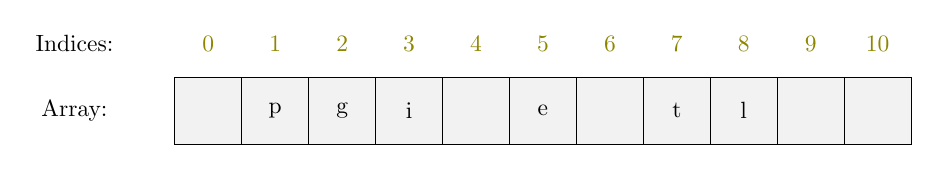
\begin{tikzpicture}[scale=0.85, transform shape]
	\foreach \x/\val in {0/,1/p,2/g,3/i,4/,5/e,6/,7/t,8/l,9/,10/}{
	\node[olive] (index) at (\x,1) {\x};
	\node[draw,rectangle, fill=gray!10, minimum size =1cm] (c) at (\x,0) {\val};
}
\node[] at (-2,1) {Indices:};
\node[] at (-2,0) {Array:};
\end{tikzpicture}

		\end{center}
	\end{block}	
	\pause
	\begin{block}{The simple mapping}
		But what if we have conflicts? Like by taking $f(k)=1$ for all $k$.
	\end{block}	
\end{frame}

\begin{frame}
	\frametitle{Hashing conflicts}
	\begin{block}{A hash table}
		We want to use hash functions to map keys to a certain index in a hash table.\\
		But what do we do if we have hashing conflicts?
	\end{block}
	\pause
	\begin{block}{Back to hundred-acre woods}
		Take $f(e) = 1$, $f(y) = 3$, $f(o) = \alert{3}$, $f(r) = 8$.
		\pause
		This would create the hash table:
		% \begin{center}
			% 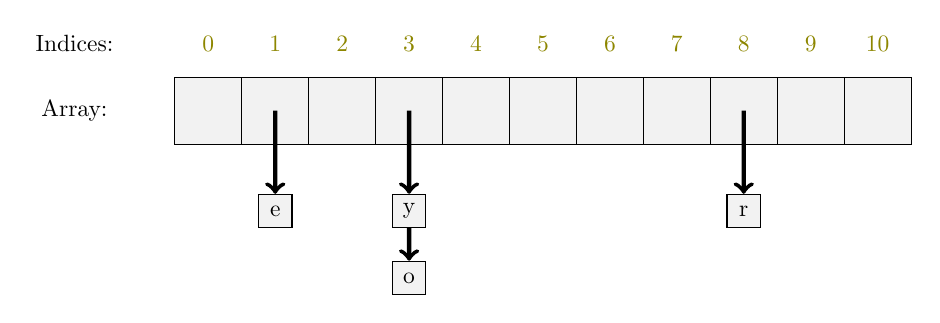
\begin{tikzpicture}[scale=0.85, transform shape]
	\foreach \x/\val in {0/,1/,2/,3/,4/,5/,6/,7/,8/,9/,10/}{
	\node[olive] (index) at (\x,1) {\x};
	\node[draw,rectangle, fill=gray!10, minimum size =1cm] (\x) at (\x,0) {\val};
}
\node[] at (-2,1) {Indices:};
\node[] at (-2,0) {Array:};

\node[draw,rectangle, fill=gray!10, minimum size =0.5cm] at (1,-1.5) (e) {e};
\node[draw,rectangle, fill=gray!10, minimum size =0.5cm] at (3,-1.5) (A) {y};
\node[draw,rectangle, fill=gray!10, minimum size =0.5cm] at (3,-2.5) (B){o};
\node[draw,rectangle, fill=gray!10, minimum size =0.5cm] at (8,-1.5) (r) {r};
\draw[->, ultra thick] (A) -- (B);
\draw[->, ultra thick] (1.center) -- (e);
\draw[->, ultra thick] (3.center) -- (A);
\draw[->, ultra thick] (8.center) -- (r);
\end{tikzpicture}

		% \end{center}
	\end{block}	
\end{frame}

\begin{frame}
	\frametitle{Hash tables}
	\begin{block}{Hash tables}
		We have an array of a certain capacity.\\
		The hash of a key, determines which \textit{bucket} to use.\\
		\pause
		Every entry could for instance hold a linked-list of values.
	\end{block}		
	\pause
	\begin{columns}
		\column{0.455\textwidth}
			
	\begin{block}{What happens?}
		So for $f(k) = 1$ for all $k$, what is the time complexity of getting the right value out for our key?
		\begin{enumerate}[A.]
			\item $\Theta(1)$
			\item $\Theta(\log n)$
			\item $\Theta(n)$
			\item $\Theta(n^2)$
		\end{enumerate}
	\end{block}
		\column{0.455\textwidth}
			
		\pause
		\begin{block}{Still linear}
			It is still linear time! All end up in a list after all.
		\end{block}
	\end{columns}
\end{frame}

\begin{frame}
	\frametitle{Hash functions: Ideal properties}
	
		\begin{block}{Hash functions}
			Hash functions map each key $k$ to a an integer in a range $[0, N-1]$ for some $N$.\\
			Where ideally:
			\pause
			\begin{itemize}
				\item keys are uniformly distributed over the range.
					\pause
				\item ($a == b) \to (\mathit{hash}(a) == \mathit{hash}(b))$ (it is deterministic).
					\pause
				\item the hash function is `fast' to compute (preferably $O(1)$).
			\end{itemize}

		\end{block}	
			\begin{block}{Rotten to the core}
				This indeed makes $f(k) = 1$ pretty terrible!
			\end{block}	
\end{frame}

\begin{frame}
	\frametitle{Implementing them in Python}
	\only<4->{\framesubtitle{Check for yourself, write a bit of code to count conflicts!}}
		\vspace{-10pt}
	\begin{columns}
		\column{0.555\textwidth}
			\lstinputlisting{src/point.py}
		\pause
		\column{0.555\textwidth}
		\lstinputlisting[firstline=4, lastline=15]{src/point2.py}
	\end{columns}
	\pause
		\vspace{-10pt}
	\begin{block}{Does it improve?}
		Which is better?	
		\vspace{-10pt}
		% \begin{multicols}{3}
		\begin{enumerate}[A.]
			\item The left one.
			\item The right one.
			\item I don't know.
		\end{enumerate}
	% \end{multicols}
	\end{block}
	\pause
		\vspace{-8pt}
		\begin{block}{It depends!}
			It depends on what kind of points we expect to see!
		\end{block}
\end{frame}


\begin{frame}
	\frametitle{Hashmaps}
	\framesubtitle{Have fun figuring out what this map represents.}
	\begin{center}
		\includegraphics[width=0.6\textwidth]{images/hashmap.png}\\
		\hspace*{15pt}\hbox{\scriptsize Image By:\thinspace{\itshape Photohound}}
	\end{center}
\end{frame}

\begin{frame}
	\frametitle{Hashmaps}
		\begin{block}{Hashmaps}
			Implement the Map ADT using Hash tables.\\
			\pause
			With a good hash function, we expect: $\Theta(1)$ insertion/deletion/retrieval.\\
			But worst-case they are still $\Theta(n)$.
		\end{block}	
		\pause
		\begin{block}{Handling hashing conflicts}
			Different options to handle hash conflicts:
			\begin{itemize}
				\item Separate Chaining
				\item (Linear) Probing
			\end{itemize}
		\end{block}
\end{frame}

\begin{frame}
	\frametitle{Lets start with the basics}
	\vspace{-13pt}
	\begin{columns}
		\column{0.355\textwidth}
		\begin{itemize}
			\item Creating a new hashmap
			\item<2-> Getting the size
			\item<3-> A hash function for keys in this map
			\item<4-> Getting an item
			\item<4-> Putting an item
		\end{itemize}
		\column{0.555\textwidth}
			
		\lstinputlisting[basicstyle=\tiny\ttfamily
		% ,linebackgroundcolor={%
			% \btLstHL<1>{3-5}%
			% \btLstHL<2>{7-8}%
			% \btLstHL<3>{10-11}%
			% \btLstHL<4>{13-15}%
			% \btLstHL<5>{17-21}%
		% }
		]
		{src/hashmap.py}
	\end{columns}
	\only<5->{
			\begin{block}{So conclusion}
				It depends on how we put things into the buckets!\\
				Do we use the linked list? Or do we do something else?
			\end{block}	
	}
\end{frame}


\begin{frame}
	\frametitle{Recap of Maps}
	
	\begin{center}
		\begin{tabular}{c | c | c}
			Operation & Expected Time & Worst-case \\
			\midrule
			\texttt{M.size()} & $\Theta(1)$& $\Theta(1)$\\
			\texttt{M.get(k)}  & $\Theta(1)$& $\Theta(n)$\\
			\texttt{M.put(k,v)} & $\Theta(1)$& $\Theta(n)$\\
			\texttt{M.remove(k)} & $\Theta(1)$& $\Theta(n)$\\
			\texttt{M.contains(k)} & $\Theta(1)$& $\Theta(n)$\\
		\end{tabular}
	\end{center}
		\begin{block}{What does this depend on?}
			It all stands or falls with the hash function!
			\begin{itemize}
				\item Fewer hash-conflicts means better performance.
				\item Separate chaining or (linear) probing does not matter for time performance.
				\item The latter saves us some space, but is not better in terms of space or time \textit{complexity}.
			\end{itemize}
		\end{block}	
\end{frame}

